% Created 2025-01-18 Sat 07:56
% Intended LaTeX compiler: pdflatex
\documentclass[11pt,oneside]{memoir}
\makeatletter

\usepackage{answerkey-env}

\ifanswerkey
  \usepackage[forcolorpaper, answerkey]{eqexam}
  \usepackage{vinaya-class-questions}
\else
  \usepackage[forcolorpaper, nosolutions]{eqexam}
  \usepackage[nosolutions]{vinaya-class-questions}
\fi

\proofingsymbolColor{linkred}
\fillinColor{linkred}

\def\maketitle{}

\maxtocdepth{subsection}

\newenvironment{twocols}{%
  \raggedright%
  \setlength{\parindent}{0pt}%
  \setlength{\parskip}{8pt}%
  \fontsize{11}{17}\selectfont%
  \begin{multicols}{2}%
}{%
  \end{multicols}%
}

\newenvironment{widecols}{%
  \hspace*{-0.05\linewidth}\begin{minipage}{1.1\linewidth}%
  \raggedright%
  \setlength{\parindent}{0pt}%
  \setlength{\parskip}{8pt}%
  \fontsize{11}{17}\selectfont%
  \begin{multicols}{2}%
}{%
  \end{multicols}%
  \end{minipage}%
}

\newlength\@tmp@width
\newlength\@tmp@height

\renewcommand*{\printchaptertitleHook}{%
  \AddToShipoutPictureBG*{%
    \put(\LenToUnit{\paperwidth-25mm-\spinemargin},\LenToUnit{\paperheight-95mm}){%
      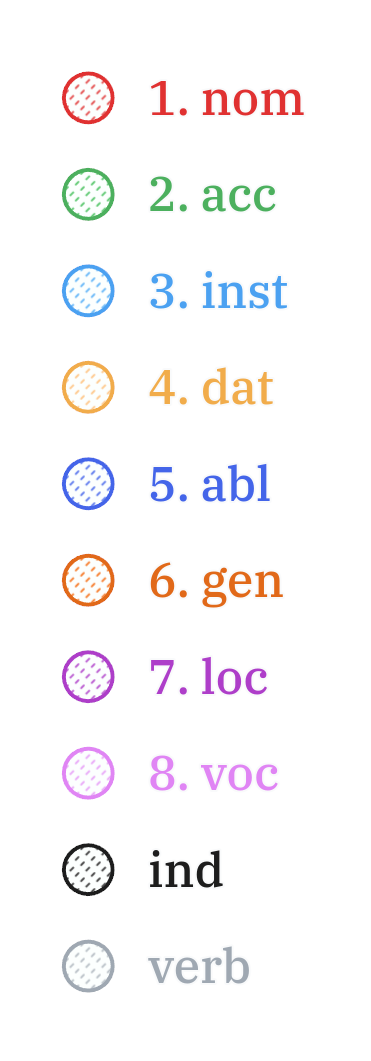
\includegraphics[width=25mm]{./images/cases-legend-white-large.png}%
    }%
  }%
}

\newcommand*\sentenceDiaMsg{\textbf{Exercise:} Draw a sentence analysis diagram below and indicate declensions.}

\newcommand*\sentenceDiaSolution[2][0.4]{%
  \ifanswerkey%
    \hspace*{-\spinemargin}%
    \begin{minipage}{\paperwidth}%
      \centering%
      \includegraphics[scale=#1]{#2}%
    \end{minipage}%
  \else%
    \settototalheight{\@tmp@height}{\includegraphics[scale=#1]{#2}}%
    \begin{minipage}[\@tmp@height]{\linewidth}%
      \sentenceDiaMsg%
    \end{minipage}%
  \fi%
}

\usepackage{cwpuzzle}

\renewcommand\PuzzleCluePre{%
  \begin{minipage}[t]{0.75\linewidth}%
}

\renewcommand\PuzzleClueFont{\fontsize{11}{17}\selectfont}

% \def\PuzzleThickline{\linethickness{2pt}}

\makeatother

\maxtocdepth{section}
\date{\today}
\title{Pāli Readings}
\hypersetup{
 pdfauthor={The Bhikkhu Saṅgha},
 pdftitle={Pāli Readings},
 pdfkeywords={},
 pdfsubject={},
 pdfcreator={Emacs 29.4 (Org mode 9.6.15)}, 
 pdflang={En_Gb}}
\begin{document}

\maketitle
\makeatletter

\newlength{\colOne}\setlength{\colOne}{0.35\linewidth}
\newlength{\colTwo}\setlength{\colTwo}{0.6\linewidth}

\renewenvironment{quote}%
{\list{}{%
    \doubleLineSize
    \listparindent 0pt
    \itemindent    0pt
    \leftmargin    3em
    \rightmargin   3em
    \parsep        0pt
    \topsep        8pt
    \partopsep     0pt}%
\item[] \raggedright}%
{\endlist}

\renewcommand*{\printchaptertitleHook}{%
  \AddToShipoutPictureBG*{%
    \put(\LenToUnit{\paperwidth-25mm-\spinemargin},\LenToUnit{\paperheight-100mm}){%
      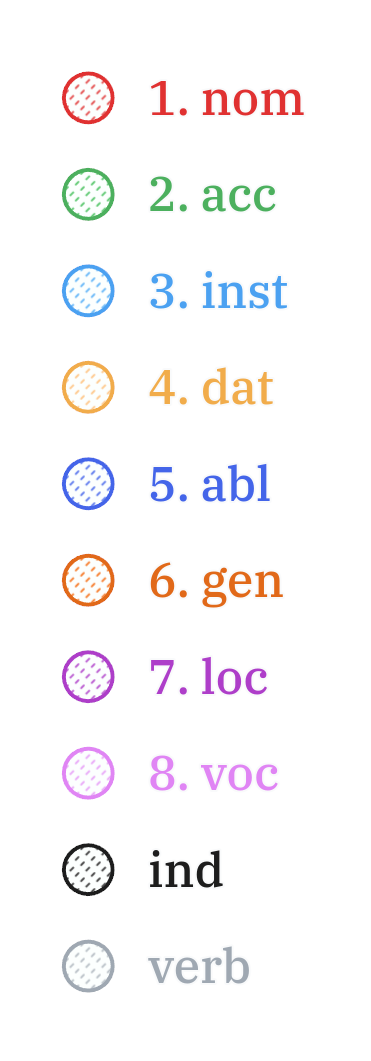
\includegraphics[width=25mm]{./images/cases-legend-white-large.png}%
    }%
  }%
}

\renewcommand*\sentenceDiaSolution[2][0.4]{%
  \ifanswerkey%
    \hspace*{-\spinemargin}%
    \begin{minipage}{\paperwidth}%
      \centering%
      \includegraphics[scale=#1]{#2}%
    \end{minipage}%
  \fi%
}

\makeatother

\mainmatter

\chapter{2025-01-22}
\label{sec:org4b1c5ce}
\section{SN 46.16 Tatiyagilānasutta}
\label{sec:org6740d50}

(\href{https://suttacentral.net/sn46.16/pli/ms}{SC}, \href{https://www.digitalpalireader.online/\_dprhtml/index.html?loc=s.4.0.0.1.1.5.m}{DPR}, \href{http://localhost:4848/suttas/sn46.16/pli/ms?window\_type=Sutta+Study}{SSP})

\begin{quote}
Ekaṁ samayaṁ bhagavā rājagahe viharati veḷuvane kalandakanivāpe.

Tena kho pana samayena bhagavā ābādhiko hoti dukkhito bāḷhagilāno.

Atha kho āyasmā mahācundo yena bhagavā tenupasaṅkami;

upasaṅkamitvā bhagavantaṁ abhivādetvā ekamantaṁ nisīdi.

Ekamantaṁ nisinnaṁ kho āyasmantaṁ mahācundaṁ bhagavā etadavoca:

“paṭibhantu taṁ, cunda, bojjhaṅgā”ti.
\end{quote}

\begin{longtable}{L{\colOne} L{\colTwo} H H}
paṭibhāti & comes to mind; occurs (to); lit. speaks back & 40689/dpd & \{\{paṭibhantu\}\} taṁ, cunda, bojjhaṅgā.\\[0pt]
√bhā & shine, speak &  & \\[0pt]
\end{longtable}

\begin{quote}
“Sattime, bhante, bojjhaṅgā \ldots{}

“Taggha, cunda, bojjhaṅgā; taggha, cunda, bojjhaṅgā”ti.

Idamavocāyasmā cundo. Samanuñño satthā ahosi. Vuṭṭhahi ca bhagavā tamhā ābādhā.

Tathāpahīno ca bhagavato so ābādho ahosī'ti.
\end{quote}

\begin{longtable}{L{\colOne} L{\colTwo} H H}
samanuñña (adj.) & approving (of); consenting (to) & 59342/dpd & \{\{Samanuñño\}\} satthā ahosi.\\[0pt]
satthā (m.) & teacher; master; the Buddha & 57894/dpd & Samanuñño \{\{satthā\}\} ahosi.\\[0pt]
\end{longtable}

\clearpage
\casesLegendHeaderBGHere

\section{Bojjhaṅga-paritta}
\label{sec:org719738f}

\begin{quote}
Bojjhaṅgo sati-saṅkhāto / dhammānaṁ vicayo tathā

Viriyam-pīti-passaddhi / bojjhaṅgā ca tathā'pare

Samādh'upekkha-bojjhaṅgā / satt'ete sabba-dassinā

Muninā sammad-akkhātā / bhāvitā bahulīkatā

Saṁvattanti abhiññāya / nibbānāya ca bodhiyā

Etena sacca-vajjena / sotthi te hotu sabbadā
\end{quote}

\begin{longtable}{L{\colOne} L{\colTwo} H H}
saṅkhāta (pp.) & reckoned; so called; pp of saṅkhāyati & 56755/dpd & bojjhaṅgo sati-\{\{saṅkhāto\}\}\\[0pt]
vicaya (m.) & investigation; examination & 67414/dpd & dhammānaṁ \{\{vicayo\}\} tathā\\[0pt]
para (pron.) & other; another & 42854/dpd & bojjhaṅgā ca tathā'\{\{pare\}\}\\[0pt]
dassī (adj.) & seeing; perceiving; knowing & 32148/dpd & sabba-\{\{dassinā\}\}\\[0pt]
muni (m.) & monk; sage; seer & 53022/dpd & \{\{muninā\}\} sammad-akkhātā\\[0pt]
vajja (ptp.) & speaking; saying; ptp of vadati & 65708/dpd & Etena sacca-\{\{vajjena\}\} sotthi te hotu sabbadā\\[0pt]
\end{longtable}

\begin{quote}
Ekasmiṁ samaye nātho / moggallānañ-ca kassapaṁ

Gilāne dukkhite disvā / bojjhaṅge satta desayi

Te ca taṁ abhinanditvā / rogā mucciṁsu taṅ-khaṇe

Etena sacca-vajjena / sotthi te hotu sabbadā
\end{quote}

\begin{longtable}{L{\colOne} L{\colTwo} H H}
nātha (m.) & protector; lord; (The Buddha) & 36192/dpd & Ekasmiṁ samaye \{\{nātho\}\}\\[0pt]
desayi (aor. +acc \& +dat) & taught (to); explained (to); aor of desayati & 33981/dpd & bojjhaṅge satta \{\{desayi\}\}\\[0pt]
mucciṁsu (aor.3rd. +abl) & was released (from); aor of muccati & 52830/dpd & rogā \{\{mucciṁsu\}\} taṅ-khaṇe\\[0pt]
khaṇa (m.) & moment; instant & 23317/dpd & rogā mucciṁsu taṅ-\{\{khaṇe\}\}\\[0pt]
\end{longtable}

\clearpage
\casesLegendHeaderBGHere

\begin{quote}
Ekadā dhamma-rājā pi / gelaññenābhipīḷito

Cundattherena tañ-ñeva / bhaṇāpetvāna sādaraṁ

Sammoditvā ca ābādhā / tamhā vuṭṭhāsi ṭhānaso

Etena sacca-vajjena / sotthi te hotu sabbadā
\end{quote}

\begin{longtable}{L{\colOne} L{\colTwo} H H}
divasa (m./nt.) & day; from diva; √div (shine) & 32680/dpd & \\[0pt]
gelañña (nt.) & sickness; ill health; [√gilā + na + *ya] & 25212/dpd & \{\{gelaññenā\}\}bhipīḷito\\[0pt]
abhipīḷita (pp.) & affected; oppressed & 7965/dpd & gelaññen\{\{ābhipīḷito\}\}\\[0pt]
taññeva (sandhi) & that very; the self same [taṁ + eva] & 29303/dpd & Cundattherena \{\{taññeva\}\}\\[0pt]
bhaṇāpeti (pr. caus.) & causes to speak; makes say; caus of bhaṇati & 49233/dpd & Cundattherena taññeva \{\{bhaṇāpetvāna\}\} sādaraṁ\\[0pt]
sādaraṁ (ind.) & with consideration; respectfully & 62172/dpd & bhaṇāpetvāna \{\{sādaraṁ\}\}\\[0pt]
sammoditvā (abs.) & having delighted together (with) [saṁ + √mud + *a + itvā] & 60932/dpd & \{\{sammoditvā\}\} ca ābādhā\\[0pt]
ṭhānaso (ind.) & on the spot; right there; lit. from the place [√ṭhā + ana + so] & 29059/dpd & tamhā vuṭṭhāsi \{\{ṭhānaso\}\}\\[0pt]
\end{longtable}

\begin{quote}
Pahīnā te ca ābādhā / tiṇṇannam-pi mahesinaṁ

Magg'āhata-kilesā va / pattānuppatti-dhammataṁ

Etena sacca-vajjena / sotthi te hotu sabbadā
\end{quote}

\begin{longtable}{L{\colOne} L{\colTwo} H H}
tiṇṇaṁ / tiṇṇannaṁ (card.) & dat. or gen. of \emph{ti} & 30430/dpd & \{\{tiṇṇannam\}\}-pi mahesinaṁ\\[0pt]
mahesi (m.) & great sage; mighty seer; [mahā + isi] & 52091/dpd & tiṇṇannam-pi \{\{mahesinaṁ\}\}\\[0pt]
āhata (pp.) & struck; beaten; destroyed; [ā + √han + ta] & 13179/dpd & Magg'\{\{āhata\}\}-kilesā va\\[0pt]
patta (pp.) & reached; attained; accomplished; pp of pāpuṇāti & 41851/dpd & \{\{pattā\}\}nuppatti-dhammataṁ\\[0pt]
anuppatti (f.) & non-arising; non-appearance; lit. not going up [ud + √pad] & 4906/dpd & patt\{\{ānuppatti\}\}-dhammataṁ\\[0pt]
dhammatā (f.) & nature; characteristic; attribute & 34714/dpd & pattānuppatti-\{\{dhammataṁ\}\}\\[0pt]
\end{longtable}

\chapter{2025-01-15}
\label{sec:org4198779}
\section{Exercise}
\label{sec:org30abd90}

\renewcommand{\arraystretch}{1.6}

\begin{center}
\begin{tabular}{lll}
word & pos & meaning\\[0pt]
\hline
samayaṁ & \fillin{3cm}{} & \fillin{5cm}{}\\[0pt]
samayena & \fillin{3cm}{} & \fillin{5cm}{}\\[0pt]
rājagahe & \fillin{3cm}{} & \fillin{5cm}{}\\[0pt]
dukkhā & \fillin{3cm}{} & \fillin{5cm}{}\\[0pt]
nibbānāya & \fillin{3cm}{} & \fillin{5cm}{}\\[0pt]
viharati & \fillin{3cm}{} & \fillin{5cm}{}\\[0pt]
upasaṅkami & \fillin{3cm}{} & \fillin{5cm}{}\\[0pt]
upasaṅkamitvā & \fillin{3cm}{} & \fillin{5cm}{}\\[0pt]
avoca & \fillin{3cm}{} & \fillin{5cm}{}\\[0pt]
saṁvattanti & \fillin{3cm}{} & \fillin{5cm}{}\\[0pt]
ahosi & \fillin{3cm}{} & \fillin{5cm}{}\\[0pt]
\end{tabular}
\end{center}

\normalArrayStretch

\section{SN 46.14 Paṭhamagilānasutta}
\label{sec:orge1f278a}

(\href{https://suttacentral.net/sn46.14/pli/ms}{SC}, \href{https://www.digitalpalireader.online/\_dprhtml/index.html?loc=s.4.0.0.1.1.3.m}{DPR}, \href{http://localhost:4848/suttas/sn46.14/pli/ms?window\_type=Sutta+Study}{SSP})

\begin{quote}
Ekaṁ samayaṁ bhagavā rājagahe viharati veḷuvane kalandakanivāpe.

Tena kho pana samayena āyasmā mahākassapo pippaliguhāyaṁ viharati

ābādhiko dukkhito bāḷhagilāno.
\end{quote}

\begin{longtable}{L{\colOne} L{\colTwo} H H}
veḷuvana (nt.) & Bamboo Grove, a park outside Rājagaha [veḷu + vana] & 70557/dpd & Ekaṁ samayaṁ bhagavā rājagahe viharati \{\{veḷuvane\}\} kalandakanivāpe.\\[0pt]
kalandaka (m.) & squirrel & 20574/dpd & Ekaṁ samayaṁ bhagavā rājagahe viharati veḷuvane \{\{kalanda\}\}kanivāpe.\\[0pt]
nivāpa (m.) & bait; fodder; feeding & 38408/dpd & Ekaṁ samayaṁ bhagavā rājagahe viharati veḷuvane kalandaka\{\{nivāpe\}\}.\\[0pt]
pippaliguhā (f.) & lit. long pepper cave [pippali + guhā] & 46161/dpd & Tena kho pana samayena āyasmā mahākassapo \{\{pippaliguhāyaṁ\}\} viharati\\[0pt]
ābādhika (adj.) & sick; ill; lit. oppressed & 11993/dpd & āyasmā mahākassapo pippaliguhāyaṁ viharati \{\{ābādhiko\}\} dukkhito bāḷhagilāno\\[0pt]
bāḷha (pp.) & very strong; extreme; intense; lit. increased [√bah + ta] & 48406/dpd & āyasmā mahākassapo pippaliguhāyaṁ viharati ābādhiko dukkhito \{\{bāḷha\}\}gilāno\\[0pt]
gilāna (adj.) & sick; ill; unwell; lit. being sick & 24950/dpd & āyasmā mahākassapo pippaliguhāyaṁ viharati ābādhiko dukkhito bāḷha\{\{gilāno\}\}\\[0pt]
\end{longtable}

\clearpage
\casesLegendHeaderBGHere

\begin{quote}
Atha kho bhagavā sāyanhasamayaṁ paṭisallānā vuṭṭhito

yenāyasmā mahākassapo tenupasaṅkami; upasaṅkamitvā paññatte āsane nisīdi.

Nisajja kho bhagavā āyasmantaṁ mahākassapaṁ etadavoca:
\end{quote}

\begin{longtable}{L{\colOne} L{\colTwo} H H}
paṭisallāna (nt.) & privacy; seclusion; solitude & 40862/dpd & Atha kho bhagavā sāyanhasamayaṁ \{\{paṭisallānā\}\} vuṭṭhito\\[0pt]
vuṭṭhita (pp. +abl) & risen (from); got up (from); pp. of vuṭṭhahati & 70020/dpd & Atha kho bhagavā sāyanhasamayaṁ paṭisallānā \{\{vuṭṭhito\}\}\\[0pt]
 & [(v) + ud + √ṭhā + ita] &  & \\[0pt]
paññatta (pp.) & prepared; arranged; lit. caused to know; & 39966/dpd & upasaṅkamitvā \{\{paññatte\}\} āsane nisīdi\\[0pt]
 & pp of paññāpeti, caus &  & \\[0pt]
\end{longtable}

\begin{quote}
“Kacci te, kassapa, khamanīyaṁ kacci yāpanīyaṁ?

Kacci dukkhā vedanā paṭikkamanti, no abhikkamanti;

paṭikkamosānaṁ paññāyati, no abhikkamo”ti?
\end{quote}

\begin{longtable}{L{\colOne} L{\colTwo} H H}
kacci (ind.) & I hope; I trust & 19264/dpd & \{\{Kacci\}\} te, kassapa, khamanīyaṁ kacci yāpanīyaṁ?\\[0pt]
khamanīya (adj.) & bearable; tolearable & 23490/dpd & Kacci te, kassapa, \{\{khamanīyaṁ\}\} kacci yāpanīyaṁ?\\[0pt]
yāpanīya (adj.) & able to keep going; sustainable & 53983/dpd & Kacci te, kassapa, khamanīyaṁ kacci \{\{yāpanīyaṁ\}\}?\\[0pt]
paṭikkamati (pr. +abl) & returns (from); comes back (from) & 40244/dpd & Kacci dukkhā vedanā \{\{paṭikkamanti\}\}, no abhikkamanti\\[0pt]
abhikkamati (pr.) & goes forward; proceeds & 7563/dpd & Kacci dukkhā vedanā paṭikkamanti, no \{\{abhikkamanti\}\}\\[0pt]
\end{longtable}

\begin{quote}
“Na me, bhante, khamanīyaṁ, na yāpanīyaṁ. Bāḷhā me dukkhā vedanā abhikkamanti,

no paṭikkamanti; abhikkamosānaṁ paññāyati, no paṭikkamo”ti.

“Sattime, kassapa, bojjhaṅgā mayā sammadakkhātā;

bhāvitā bahulīkatā abhiññāya sambodhāya nibbānāya saṁvattanti. Katame satta?

Satisambojjhaṅgo kho, kassapa, mayā sammadakkhāto bhāvito bahulīkato

abhiññāya sambodhāya nibbānāya saṁvattati \ldots{} Ime kho, kassapa, satta bojjhaṅgā \ldots{}

“Taggha, bhagavā, bojjhaṅgā; taggha, sugata, bojjhaṅgā”ti.
\end{quote}

\begin{longtable}{L{\colOne} L{\colTwo} H H}
sammadakkhāta (adj.) & well taught; well preached [sammā + (d) + akkhāta] & 60730/dpd & Sattime, kassapa, bojjhaṅgā mayā \{\{sammadakkhātā\}\}; bhāvitā bahulīkatā\\[0pt]
akkhāta (pp. +instr) & said (by); declared (by) & 399/dpd & Sattime, kassapa, bojjhaṅgā mayā sammad\{\{akkhātā\}\}; bhāvitā bahulīkatā\\[0pt]
bahulīkata (pp.) & practised often; repeated a lot; [bahula + kata] & 48190/dpd & Sattime, kassapa, bojjhaṅgā mayā sammadakkhātā; bhāvitā \{\{bahulīkatā\}\}\\[0pt]
taggha (ind.) & truly; definitely; lit. that indeed [tad + gha] & 29228/dpd & \{\{Taggha\}\}, bhagavā, bojjhaṅgā\\[0pt]
\end{longtable}

\clearpage
\casesLegendHeaderBGHere

\begin{quote}
Idamavoca bhagavā. Attamano āyasmā mahākassapo bhagavato bhāsitaṁ abhinandi.

Vuṭṭhahi cāyasmā mahākassapo tamhā ābādhā.

Tathāpahīno cāyasmato mahākassapassa so ābādho ahosī'ti.
\end{quote}

\begin{longtable}{L{\colOne} L{\colTwo} H H}
attamana (adj.) & pleased; satisfied; lit. own mind [atta + mana] & 2524/dpd & \{\{Attamano\}\} āyasmā mahākassapo bhagavato bhāsitaṁ abhinandi.\\[0pt]
vuṭṭhahi (aor. +abl) & arose (from); got up (from); recovered (from) & 69980/dpd & \{\{Vuṭṭhahi\}\} cāyasmā mahākassapo tamhā ābādhā.\\[0pt]
tamhā (pron.) & from that [ta + mhā] masc \& nt abl sg of ta & 30060/dpd & Vuṭṭhahi cāyasmā mahākassapo \{\{tamhā\}\} ābādhā.\\[0pt]
pahīna (pp.) & abandoned; dispelled; pp. of pajahati & 45133/dpd & Tathā\{\{pahīno\}\} cāyasmato mahākassapassa so ābādho ahosī'ti.\\[0pt]
\end{longtable}

\section{SN 46.15 Dutiyagilānasutta}
\label{sec:orga107a5c}

(\href{https://suttacentral.net/sn46.15/pli/ms}{SC}, \href{https://www.digitalpalireader.online/\_dprhtml/index.html?loc=s.4.0.0.1.1.4.m}{DPR}, \href{http://localhost:4848/suttas/sn46.15/pli/ms?window\_type=Sutta+Study}{SSP})

\begin{quote}
Ekaṁ samayaṁ bhagavā rājagahe viharati veḷuvane kalandakanivāpe.
Tena kho pana samayena āyasmā mahāmoggallāno gijjhakūṭe pabbate viharati
ābādhiko dukkhito bāḷhagilāno.
\end{quote}

\begin{longtable}{L{\colOne} L{\colTwo} H H}
gijjhakūṭa (m.) & Vulture's Peak [gijjha + kūṭa] & 24890/dpd & āyasmā mahāmoggallāno \{\{gijjhakūṭe\}\} pabbate viharati\\[0pt]
pabbata (m.) & rock; mountain; hill & 42495/dpd & āyasmā mahāmoggallāno gijjhakūṭe \{\{pabbate\}\} viharati\\[0pt]
\end{longtable}

\textbf{Bojjhaṅga-paritta:}

\begin{quote}
Ekasmiṁ samaye nātho

moggallānañ-ca kassapaṁ

Gilāne dukkhite disvā

bojjhaṅge satta desayi

Te ca taṁ abhinanditvā

rogā mucciṁsu taṅkhaṇe

Etena sacca-vajjena

sotthi te hotu sabbadā
\end{quote}

\chapter{2025-01-08}
\label{sec:orgda2106e}
\section{Declension Cases Overview}
\label{sec:org42d1dd1}

\begin{tabular}{lll}
1. Nominative & subject performing the action & Who is giving?\\[0pt]
2. Accusative & direct object & What is he/she giving?\\[0pt]
3. Instrumental & means, instrument & With/by/through what?\\[0pt]
4. Dative & indirect object, recipient, purpose & To whom? For what?\\[0pt]
5. Ablative & motion/separation from, comparison & From where? Better than what?\\[0pt]
6. Genitive & possession, relationship & Whose?\\[0pt]
7. Locative & location, time & Where? When?\\[0pt]
8. Vocative & direct address & Form, bhikkhus, is not-self.\\[0pt]
\end{tabular}

\bigskip {\centering
Mnemonics:
\par}

\begin{center}
\begin{tabular}{ll}
1. \textbf{Nominate} who will do it. & 5. Pieces fall from the \textbf{ablative} heat-shield.\\[0pt]
2. Give an objective \textbf{accusation}. & 6. The \textbf{genitive} glues possessions to people.\\[0pt]
3. Fix it with this \textbf{instrument}. & 7. \textbf{Locate} him in space and time.\\[0pt]
4. \textbf{Donate} a date to him. & 8. Shout a \textbf{vocal} address.\\[0pt]
\end{tabular}
\end{center}

Origin of the word `Dative':

\begin{center}
\begin{tabular}{ll}
PIE root: & \emph{√do-} to give\\[0pt]
Latin: & \emph{donum} gift, \emph{donatio} a giving, \emph{dativus} pertaining to giving\\[0pt]
Pāli/Sanskrit: & \emph{dadāti} gives [√dā + dā + a → dadā]\\[0pt]
\end{tabular}
\end{center}

Origin of the word `Ablative':

\begin{center}
\begin{tabular}{lllll}
Latin & PIE & Pāli/Sanskrit &  & \\[0pt]
\emph{ab-} & \emph{√apo} & \emph{apa-} & off, away from & apocalypse, apology, apostle\\[0pt]
\emph{ferre} & \emph{√bher-} & \emph{√bhar} / \emph{√bhṛ} & to carry, to bear & birth, bring, burden,\\[0pt]
 &  &  &  & differ, offer, suffer, transfer\\[0pt]
\end{tabular}
\end{center}

\clearpage

\section{Cases Exercise: The Elephant}
\label{sec:org68ecf98}

\casesLegendHeaderBGHere

\begin{quote}
Jetavane hatthinī soṇḍāya vā dīghahatthena vā

attano hatthipotakassa tiṇaṁ datvā,

tato soṇḍato mahāsaddaṁ pahiṇi.

Imassa hatthipotakassa tiṇena kucchi mahanto ahosi.
\end{quote}

\bigskip

\begin{center}
\begin{tabular}{llll}
hatthinī (f.) & female elephant [hatthī + inī] & pahiṇi (aor.) & sent; aor. of pahiṇāti\\[0pt]
soṇḍā (f.) & elephant's trunk & kucchi (m.) & stomach; belly\\[0pt]
hattha (m.) & hand & mahanta (adj.) & big; large\\[0pt]
potaka (m.) & young animal & ahosi (aor.) & was; became; aor. of hoti\\[0pt]
tiṅa (nt.) & grass; straw &  & \\[0pt]
\end{tabular}
\end{center}

\enlargethispage{\baselineskip}
\renewcommand{\arraystretch}{1.6}

\begin{center}
\begin{tabular}{lll}
word & meaning & case\\[0pt]
\hline
Jetavane & \fillin{5cm}{at Jetavana} & \fillin{3cm}{loc.}\\[0pt]
hatthinī & \fillin{5cm}{the female elephant} & \fillin{3cm}{nom.}\\[0pt]
soṇḍāya vā & \fillin{5cm}{by the trunk} & \fillin{3cm}{inst.}\\[0pt]
dīghahatthena vā & \fillin{5cm}{or by the long hand} & \fillin{3cm}{inst.}\\[0pt]
attano & \fillin{5cm}{her own} & \fillin{3cm}{gen.}\\[0pt]
hatthipotakassa & \fillin{5cm}{to the baby-elephant} & \fillin{3cm}{dat.}\\[0pt]
tiṇaṁ & \fillin{5cm}{grass} & \fillin{3cm}{acc.}\\[0pt]
datvā & \fillin{5cm}{having given} & \fillin{3cm}{ger.}\\[0pt]
tato & \fillin{5cm}{then} & \fillin{3cm}{ind.}\\[0pt]
soṇḍato & \fillin{5cm}{from the trunk} & \fillin{3cm}{abl.}\\[0pt]
mahāsaddaṁ & \fillin{5cm}{a loud noise} & \fillin{3cm}{acc.}\\[0pt]
pahiṇi & \fillin{5cm}{sent (→ pahiṇāti)} & \fillin{3cm}{aor.}\\[0pt]
imassa & \fillin{5cm}{pron. of this (→ ima)} & \fillin{3cm}{gen.sg.}\\[0pt]
hatthipotakassa & \fillin{5cm}{of the baby elephant} & \fillin{3cm}{gen.}\\[0pt]
tiṇena & \fillin{5cm}{with grass} & \fillin{3cm}{inst.}\\[0pt]
kucchi & \fillin{5cm}{belly, stomach} & \fillin{3cm}{nom.}\\[0pt]
mahanto & \fillin{5cm}{adj. great, large} & \fillin{3cm}{nom.}\\[0pt]
ahosi & \fillin{5cm}{was, became (→ hoti)} & \fillin{3cm}{aor.}\\[0pt]
\end{tabular}
\end{center}

\normalArrayStretch

\clearpage

\section{AN 10.81 Vāhanasutta, The lotus simile to Vāhana}
\label{sec:orgfaa8d1f}
\casesLegendHeaderBGHere

(\href{https://suttacentral.net/an10.81/pli/ms}{SC}, \href{https://www.digitalpalireader.online/\_dprhtml/index.html?loc=a.9.0.0.1.3.0.m}{DPR}, \href{http://localhost:4848/suttas/an10.81/pli/ms?window\_type=Sutta+Study}{SSP}, Nibbāna Sermon 18)

\begin{quote}
Ekaṁ samayaṁ bhagavā campāyaṁ viharati gaggarāya pokkharaṇiyā tīre.

Atha kho āyasmā vāhano yena bhagavā tenupasaṅkami;

upasaṅkamitvā bhagavantaṁ abhivādetvā ekamantaṁ nisīdi.

Ekamantaṁ nisinno kho āyasmā vāhano bhagavantaṁ etadavoca:
\end{quote}

\begin{longtable}{L{\colOne} L{\colTwo} H H}
pokkhara (nt.) & blue lotus flower & 47383/dpd & Ekaṁ samayaṁ bhagavā campāyaṁ viharati gaggarāya \{\{pokkharaṇiyā\}\} tīre.\\[0pt]
tīra (nt.) & shore, riverbank & 30918/dpd & Ekaṁ samayaṁ bhagavā campāyaṁ viharati gaggarāya pokkharaṇiyā \{\{tīre\}\}.\\[0pt]
yena \ldots{} ten'upasaṅkamati (idiom) & wherever \ldots{} he approaches (him/it) & 31234/dpd & Atha kho āyasmā vāhano yena bhagavā \{\{tenupasaṅkami\}\}\\[0pt]
abhivādeti & bows down (to); pays high respect (to) & 8333/dpd & upasaṅkamitvā bhagavantaṁ \{\{abhivādetvā\}\} ekamantaṁ nisīdi.\\[0pt]
ekamantaṁ (ind.) & to one side; aside [ekaṁ + anta + aṁ] & 17613/dpd & upasaṅkamitvā bhagavantaṁ abhivādetvā \{\{ekamantaṁ\}\} nisīdi.\\[0pt]
nisīdati & sits (on); sits down & 38204/dpd & upasaṅkamitvā bhagavantaṁ abhivādetvā ekamantaṁ \{\{nisīdi\}\}.\\[0pt]
avoca (aor.) & said (to); aor. of vacati & 10795/dpd & āyasmā vāhano bhagavantaṁ etad\{\{avoca\}\}\\[0pt]
\end{longtable}

\begin{quote}
“Katihi nu kho, bhante, dhammehi tathāgato nissaṭo visaṁyutto vippamutto

vimariyādīkatena cetasā viharatī”ti?
\end{quote}

\begin{longtable}{L{\colOne} L{\colTwo} H H}
kati (interr.) & how many? & 19695/dpd & \{\{Katihi\}\} nu kho, bhante, dhammehi tathāgato nissaṭo\\[0pt]
nissaṭa (pp. +abl) & escaped (from), freed (from); pp. of nissarati & 38271/dpd & tathāgato \{\{nissaṭo\}\} visaṁyutto vippamutto vimariyādīkatena cetasā viharati\\[0pt]
visaṁyutta (pp. +abl) & detached (from) & 69208/dpd & tathāgato nissaṭo \{\{visaṁyutto\}\} vippamutto vimariyādīkatena cetasā viharati\\[0pt]
vippamutta (pp. +abl) & released (from) & 68475/dpd & tathāgato nissaṭo visaṁyutto \{\{vippamutto\}\} vimariyādīkatena cetasā viharati\\[0pt]
vimariyādīkata (adj.) & unbounded [vi + mariyādā + kata] & 68663/dpd & tathāgato nissaṭo visaṁyutto vippamutto \{\{vimariyādīkatena\}\} cetasā viharati\\[0pt]
mariyādā (f.) & boundary, border, limit & 51492/dpd & tathāgato nissaṭo visaṁyutto vippamutto vi\{\{mariyādī\}\}katena cetasā viharati\\[0pt]
\end{longtable}

\begin{quote}
“Dasahi kho, vāhana, dhammehi tathāgato nissaṭo visaṁyutto vippamutto vimariyādīkatena

cetasā viharati. Katamehi dasahi? Rūpena kho, vāhana, tathāgato nissaṭo visaṁyutto

vippamutto vimariyādīkatena cetasā viharati, vedanāya \ldots{} saññāya \ldots{} saṅkhārehi \ldots{} viññāṇena

\ldots{} jātiyā \ldots{} jarāya \ldots{} maraṇena \ldots{} dukkhehi \ldots{} kilesehi kho, vāhana, tathāgato nissaṭo

visaṁyutto vippamutto vimariyādīkatena cetasā viharati.
\end{quote}

\clearpage
\casesLegendHeaderBGHere

\begin{quote}
Seyyathāpi, vāhana, uppalaṁ vā padumaṁ vā puṇḍarīkaṁ vā

udake jātaṁ udake saṁvaḍḍhaṁ udakā paccuggamma ṭhitaṁ anupalittaṁ udakena;

evamevaṁ kho, vāhana, imehi dasahi dhammehi tathāgato nissaṭo visaṁyutto

vippamutto vimariyādīkatena cetasā viharatī”ti.
\end{quote}

\begin{longtable}{L{\colOne} L{\colTwo} H H}
uppala, paduma, puṇḍarīka (nt.) & types of lotus & 16618/dpd & Seyyathāpi, vāhana, \{\{uppalaṁ\}\} vā padumaṁ vā puṇḍarīkaṁ vā\\[0pt]
udaka (nt.) & water & 14832/dpd & \{\{udake\}\} jātaṁ \{\{udake\}\} saṁvaḍḍhaṁ \{\{udakā\}\} paccuggamma ṭhitaṁ anupalittaṁ \{\{udakena\}\}\\[0pt]
saṁvaḍḍha (pp.) & grown up (in); fully grown (in) [saṁ + √vaḍḍh + ta] & 61844/dpd & udake jātaṁ udake \{\{saṁvaḍḍhaṁ\}\} udakā paccuggamma ṭhitaṁ anupalittaṁ udakena\\[0pt]
paccuggamma (ger. +abl) & going out (from), emerging (from); ger of paccuggacchati & 39489/dpd & udake jātaṁ udake saṁvaḍḍhaṁ udakā \{\{paccuggamma\}\} ṭhitaṁ anupalittaṁ udakena\\[0pt]
tiṭṭhati & stands & 30486/dpd & udake jātaṁ udake saṁvaḍḍhaṁ udakā paccuggamma \{\{ṭhitaṁ\}\} anupalittaṁ udakena\\[0pt]
anupalitta (pp. +instr) & not smeared (by), untainted (by); [na + upalitta] & 4747/dpd & udake jātaṁ udake saṁvaḍḍhaṁ udakā paccuggamma ṭhitaṁ \{\{anupalittaṁ\}\} udakena\\[0pt]
\end{longtable}

\section{MN 112, The bhikkhu with defilements ended}
\label{sec:org78ea993}

(See also: Nibbāna Sermon 15)

\begin{quote}
Khīṇāsavassa, bhikkhave, bhikkhuno \ldots{} veyyākaraṇāya:

`Diṭṭhe kho ahaṁ, āvuso, anupāyo anapāyo anissito appaṭibaddho vippamutto
visaṁyutto vimariyādīkatena cetasā viharāmi.'

`Sute \ldots{} mute \ldots{} viññāte \ldots{}'
\end{quote}
\end{document}
